\documentclass[aspectratio=169,10pt]{beamer}

% Shared Beamer setup for Fall 2026 course slides.
% Clean Cal Poly-inspired theme: no custom class files or uncommon packages.
\mode<presentation>{
  \usetheme{default}
  \usefonttheme{professionalfonts}
}

\definecolor{CalPolyGreen}{HTML}{154734}
\definecolor{CalPolyGold}{HTML}{BD8B13}
\definecolor{CalPolySage}{HTML}{7FA28F}
\definecolor{CalPolyMint}{HTML}{DDF1E7}
\definecolor{CalPolySand}{HTML}{A29F86}
\definecolor{CalPolyBeige}{HTML}{EFEEDE}
\definecolor{DeckInk}{HTML}{1F2933}
\definecolor{DeckMuted}{HTML}{5F6B7A}
\definecolor{DeckSoft}{HTML}{F7F7F5}

\setbeamersize{text margin left=0.55in,text margin right=0.55in}
\setbeamercolor{normal text}{fg=DeckInk,bg=white}
\setbeamercolor{structure}{fg=CalPolyGreen}
\setbeamercolor{title}{fg=white}
\setbeamercolor{frametitle}{fg=CalPolyGreen,bg=white}
\setbeamercolor{block title}{bg=CalPolySage,fg=white}
\setbeamercolor{block body}{bg=CalPolyMint,fg=black}
\setbeamercolor{alerted text}{fg=CalPolyGold}

\setbeamerfont{title}{size=\Huge,series=\bfseries}
\setbeamerfont{frametitle}{size=\Large,series=\bfseries}
\setbeamerfont{block title}{size=\normalsize,series=\bfseries}

\setbeamertemplate{navigation symbols}{}
\setbeamertemplate{itemize item}{\color{CalPolyGold}$\blacktriangleright$}
\setbeamertemplate{itemize subitem}{\color{CalPolyGreen}$\bullet$}
\setbeamertemplate{footline}{
  \hfill{\color{DeckMuted}\scriptsize\insertframenumber/\inserttotalframenumber}
  \hspace{0.18in}\vspace{0.12in}
}
\setbeamertemplate{frametitle}{
  \vspace{0.18in}
  \hspace{0.02in}\insertframetitle\par
  \vspace{0.08in}
  \noindent\makebox[\linewidth][l]{%
    {\color{CalPolyGold}\rule{0.55in}{2pt}}%
    {\color{CalPolyGreen}\rule{\dimexpr\linewidth-0.55in\relax}{2pt}}%
  }
}

\newcommand{\CourseNumber}{Course}
\newcommand{\CourseTitle}{Course Title}
\newcommand{\LectureNumber}{0}
\newcommand{\LectureTitle}{Lecture Title}
\newcommand{\LectureDate}{Date}
\newcommand{\CourseUnit}{Unit}

\newcommand{\coursenumber}[1]{\renewcommand{\CourseNumber}{#1}}
\newcommand{\coursetitle}[1]{\renewcommand{\CourseTitle}{#1}}
\newcommand{\lecturenumber}[1]{\renewcommand{\LectureNumber}{#1}}
\newcommand{\lecturetitle}[1]{\renewcommand{\LectureTitle}{#1}}
\newcommand{\lecturedate}[1]{\renewcommand{\LectureDate}{#1}}
\newcommand{\courseunit}[1]{\renewcommand{\CourseUnit}{#1}}

\author{Kirk Duran}
\institute{California Polytechnic State University, San Luis Obispo}
\date{\LectureDate}

\newcommand{\makedecktitle}{
  \begingroup
  \setbeamercolor{background canvas}{bg=CalPolyGreen}
  \begin{frame}[plain]
    \vfill
    \begin{center}
      {\usebeamerfont{title}\color{white}\LectureTitle\par}
      \vspace{0.18in}
      {\Large\color{white}Lecture \LectureNumber\par}
    \end{center}
    \vfill
    \noindent{\color{white}\rule{\linewidth}{1.2pt}}\par
    \vspace{0.08in}
    \noindent\colorbox{CalPolyGold}{\makebox[0.24\linewidth][c]{\color{white}\Large\CourseNumber}}
    \hspace{0.12in}{\color{white}\Large Kirk Duran}
  \end{frame}
  \endgroup
}

\newenvironment{keyidea}{\begin{block}{Key idea}}{\end{block}}
\newenvironment{activity}{\begin{block}{In class}}{\end{block}}
\newenvironment{cpdefinition}{\begin{block}{Definition}}{\end{block}}
\newenvironment{exampleblockcp}{
  \begingroup
  \setbeamercolor{block title}{bg=CalPolySand,fg=white}
  \setbeamercolor{block body}{bg=CalPolyBeige,fg=black}
  \begin{block}{Example}
}{
  \end{block}
  \endgroup
}

\newcommand{\imageplaceholder}[2][0.3in]{%
  \noindent\makebox[\linewidth][c]{%
    \fcolorbox{CalPolySage}{CalPolyBeige}{%
      \parbox[c][#1][c]{0.86\linewidth}{%
        \centering
        {\color{DeckMuted}\scriptsize Image placeholder: }%
        {\color{DeckInk}\scriptsize\ttfamily\detokenize{#2}}%
      }%
    }%
  }%
}

\newcommand{\sectionframe}[1]{
  \begingroup
  \setbeamercolor{background canvas}{bg=CalPolyGreen}
  \begin{frame}[plain]
    \vfill
    {\color{white}\LARGE\bfseries #1\par}
    \vspace{0.18in}
    {\color{CalPolyGold}\rule{0.22\paperwidth}{3pt}}
    {\color{white}\rule{0.62\paperwidth}{3pt}}
    \vfill
  \end{frame}
  \endgroup
}

\newcommand{\placeholdernote}{
  \begin{block}{Placeholder}
    Replace these bullets with the final lecture material, examples, and in-class activities.
  \end{block}
}


\usepackage{tikz}
\usetikzlibrary{arrows.meta,positioning,shapes.geometric,calc}

\graphicspath{{../assets/lecture-23/}}

\newcommand{\lectureimage}[2][1.75in]{%
  \IfFileExists{../assets/lecture-23/#2}{%
    \includegraphics[width=\linewidth,height=#1,keepaspectratio]{#2}%
  }{}%
}

\newcommand{\lectureplaceholder}[2][2.35in]{%
  \begin{center}
    \fbox{%
      \begin{minipage}[c][#1][c]{0.90\linewidth}
        \centering
        \small\textit{#2}
      \end{minipage}%
    }
  \end{center}%
}

\setbeamersize{text margin left=0.42in,text margin right=0.42in}

\coursenumber{CS 4880}
\coursetitle{Artificial Intelligence}
\lecturenumber{23}
\lecturetitle{Markov Decision Processes and Partial Observability}
\lecturedate{October 19, 2026}
\courseunit{Temporal and Decision Reasoning}

\begin{document}

% Estimated pacing: 50--55 minutes
% MDP motivation and formalism: 14 min
% Value functions and dynamic programming: 16 min
% Limits of full observability + POMDP pivot: 10 min
% POMDP blow-up + Monte Carlo circle-back: 10--15 min

% -----------------------------------------------------------------------------
% Slide 1
% -----------------------------------------------------------------------------
\makedecktitle

\section{From Myopic Decisions to Sequential Decisions}

% -----------------------------------------------------------------------------
% Slide 2
% -----------------------------------------------------------------------------
\begin{frame}[shrink=10]{Last Time: One-Step Decision Making}
  The robot combined three ingredients:
  \begin{itemize}
    \item a belief about the current world;
    \item a utility model over outcomes;
    \item expected utility to choose the best action now.
  \end{itemize}

  \[
    a^*=\arg\max_a EU(a)
  \]

  \begin{keyidea}
    Decision networks solved ``what should I do now?'' but did not yet reason about how today's action changes tomorrow's choices.
  \end{keyidea}
\end{frame}

% -----------------------------------------------------------------------------
% Slide 3
% -----------------------------------------------------------------------------
\begin{frame}[shrink=10]{The Problem: A Locally Good Action Can Create a Bad Future}
  \begin{columns}[T,onlytextwidth]
    \begin{column}{0.47\textwidth}
      \begin{block}{Shortcut now}
        Immediate reward: $+6$.

        Fast if the plaza stays clear, but entering it may trap the robot behind dense pedestrian traffic.
      \end{block}
    \end{column}
    \begin{column}{0.47\textwidth}
      \begin{block}{Detour now}
        Immediate reward: $+2$.

        Slower right now, but it moves the robot into a predictable corridor with many good future choices.
      \end{block}
    \end{column}
  \end{columns}

  \begin{keyidea}
    The quality of an action depends on both its immediate outcome and the future states it makes likely.
  \end{keyidea}
\end{frame}

% -----------------------------------------------------------------------------
% Slide 4
% -----------------------------------------------------------------------------
\begin{frame}[shrink=10]{This Is No Longer Just a Path Problem}
  A path is a fixed sequence:
  \[
    North, North, East, East, \ldots
  \]

  But the robot does not control exactly what happens after each move.
  \begin{itemize}
    \item pedestrians change motion;
    \item doors may open or close;
    \item wheel slip changes position;
    \item congestion changes what is reachable next.
  \end{itemize}

  \lectureimage[1.6in]{slide4.png}

  \begin{keyidea}
    We need a policy---a decision rule that reacts to the state reached, not a single precomputed path.
  \end{keyidea}
\end{frame}

% -----------------------------------------------------------------------------
% Slide 5
% -----------------------------------------------------------------------------
\begin{frame}[shrink=10]{The MDP Loop}
  \begin{center}
    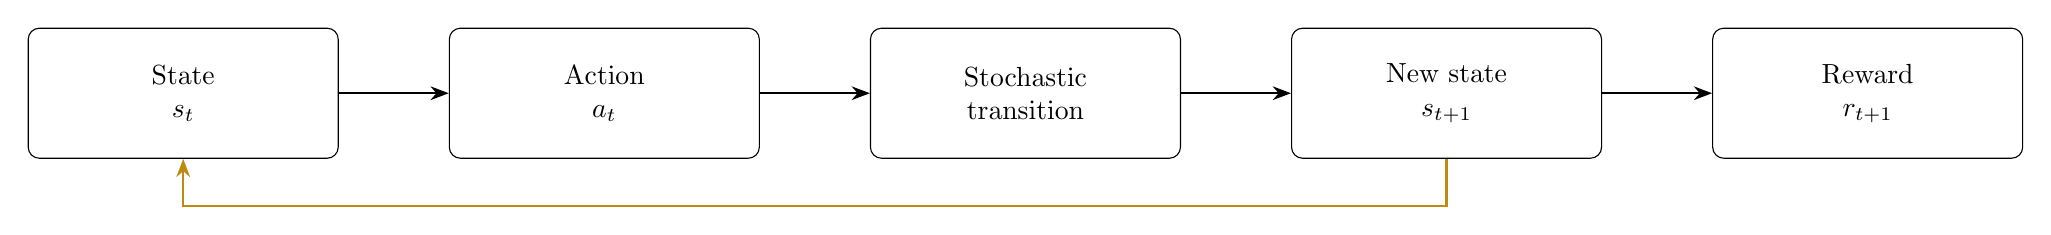
\begin{tikzpicture}[node distance=0.55in,every node/.style={draw,rounded corners,align=center,minimum width=1.55in,minimum height=0.65in}]
      \node (s) {State\\$s_t$};
      \node[right=of s] (a) {Action\\$a_t$};
      \node[right=of a] (t) {Stochastic\\transition};
      \node[right=of t] (sp) {New state\\$s_{t+1}$};
      \node[right=of sp] (r) {Reward\\$r_{t+1}$};
      \draw[-{Stealth},thick] (s)--(a);
      \draw[-{Stealth},thick] (a)--(t);
      \draw[-{Stealth},thick] (t)--(sp);
      \draw[-{Stealth},thick] (sp)--(r);
      \draw[-{Stealth},thick,CalPolyGold] (sp.south) |- ++(0,-0.6) -| (s.south);
    \end{tikzpicture}
  \end{center}

  \begin{keyidea}
    A Markov Decision Process formalizes repeated decision making when actions have uncertain consequences and future rewards matter.
  \end{keyidea}
\end{frame}

\section{Markov Decision Processes}

% -----------------------------------------------------------------------------
% Slide 6
% -----------------------------------------------------------------------------
\begin{frame}[shrink=10]{A Markov Decision Process}
  \[
    \boxed{MDP=(S,A,T,R,\gamma)}
  \]

  \begin{center}
    \renewcommand{\arraystretch}{1.3}
    \begin{tabular}{c|p{0.72\textwidth}}
      $S$ & states: what situation is the robot in? \\
      $A$ & actions: what can the robot do? \\
      $T$ & transition model: where might an action lead? \\
      $R$ & reward: what immediate feedback is produced? \\
      $\gamma$ & discount factor: how strongly do future rewards matter? \\
    \end{tabular}
  \end{center}

  \begin{keyidea}
    An MDP separates the world model from the decision objective, then connects them through a policy.
  \end{keyidea}
\end{frame}

% -----------------------------------------------------------------------------
% Slide 7
% -----------------------------------------------------------------------------
\begin{frame}[shrink=10]{What Counts as a State?}
  A useful robot state might include:
  \begin{itemize}
    \item location or campus region;
    \item battery band;
    \item remaining delivery task;
    \item whether a door is open;
    \item congestion level if it changes future transitions.
  \end{itemize}

  The Markov property is
  \[
    P(s_{t+1}\mid s_t,a_t,\text{history})
    =P(s_{t+1}\mid s_t,a_t).
  \]

  \begin{keyidea}
    ``State'' is an engineering abstraction: include what matters for predicting the future, omit what does not.
  \end{keyidea}
\end{frame}

% -----------------------------------------------------------------------------
% Slide 8
% -----------------------------------------------------------------------------
\begin{frame}[shrink=10]{State Design Is Already a Tradeoff}
  \begin{columns}[T,onlytextwidth]
    \begin{column}{0.47\textwidth}
      \begin{block}{State too small}
        If state is only location, but battery changes which moves are safe, then two visits to the ``same'' state can have different futures.

        The model is not truly Markov.
      \end{block}
    \end{column}
    \begin{column}{0.47\textwidth}
      \begin{block}{State too rich}
        Location $\times$ battery $\times$ task $\times$ crowd density $\times$ weather $\times$ door status $\times \cdots$

        Prediction improves, but the number of states explodes.
      \end{block}
    \end{column}
  \end{columns}

  \begin{keyidea}
    Markov state design trades model fidelity against state-space size.
  \end{keyidea}
\end{frame}

% -----------------------------------------------------------------------------
% Slide 9
% -----------------------------------------------------------------------------
\begin{frame}[shrink=10]{Actions Are the Robot's Controllable Choices}
  The action set might include:
  \begin{itemize}
    \item move forward, turn, backtrack;
    \item wait for traffic to move;
    \item perform a slower scan or re-localize;
    \item deliver the package;
    \item dock or request assistance.
  \end{itemize}

  \begin{keyidea}
    The action set defines what control authority the agent actually has.
  \end{keyidea}
\end{frame}

% -----------------------------------------------------------------------------
% Slide 10
% -----------------------------------------------------------------------------
\begin{frame}[shrink=10]{The Transition Model Makes Actions Stochastic}
  \[
    T(s,a,s')=P(s_{t+1}=s'\mid s_t=s,a_t=a)
  \]

  Example from the campus intersection:
  \begin{center}
    \renewcommand{\arraystretch}{1.3}
    \begin{tabular}{l|l}
      \textbf{Action} & \textbf{Possible next states} \\\hline
      Shortcut & $0.70$ NearGoal, $0.25$ CrowdedPlaza, $0.05$ SameLocation \\
      Detour & $0.95$ SafeCorridor, $0.05$ SameLocation \\
      Wait & $0.60$ CrowdClears, $0.40$ CrowdPersists \\
    \end{tabular}
  \end{center}

  \begin{keyidea}
    The robot chooses the action, not the outcome.
  \end{keyidea}
\end{frame}

% -----------------------------------------------------------------------------
% Slide 11
% -----------------------------------------------------------------------------
\begin{frame}[shrink=10]{Reward Is Immediate; Return Is Long-Term}
  \begin{columns}[T,onlytextwidth]
    \begin{column}{0.47\textwidth}
      \begin{block}{Reward $R_t$}
        Feedback for one transition.
        \begin{itemize}
          \item $+20$ deliver package
          \item $-1$ each time step
          \item $-8$ enter dense crowd
          \item $-100$ collision
        \end{itemize}
      \end{block}
    \end{column}
    \begin{column}{0.47\textwidth}
      \begin{block}{Return $G_t$}
        Accumulated reward produced by a sequence of future decisions.

        A move can be mediocre now but create a much better long-term future.
      \end{block}
    \end{column}
  \end{columns}

  \begin{keyidea}
    MDPs optimize a trajectory of consequences, not the next reward in isolation.
  \end{keyidea}
\end{frame}

% -----------------------------------------------------------------------------
% Slide 12
% -----------------------------------------------------------------------------
\begin{frame}[shrink=10]{Discounted Return}
  \[
    G_t=R_{t+1}+\gamma R_{t+2}+\gamma^2R_{t+3}+\cdots
  \]

  \begin{itemize}
    \item $\gamma=0$: only the next reward matters.
    \item $0<\gamma<1$: future rewards matter but are progressively discounted.
    \item $\gamma\approx1$: long-run consequences matter strongly.
  \end{itemize}

  \begin{keyidea}
    The discount factor controls how strongly delayed consequences influence current actions.
  \end{keyidea}
\end{frame}

% -----------------------------------------------------------------------------
% Slide 13
% -----------------------------------------------------------------------------
\begin{frame}[shrink=10]{What Does the Discount Factor Mean for the Robot?}
  \begin{columns}[T,onlytextwidth]
    \begin{column}{0.30\textwidth}
      \begin{block}{Time preference}
        Earlier task completion may be operationally more valuable.
      \end{block}
    \end{column}
    \begin{column}{0.30\textwidth}
      \begin{block}{Future uncertainty}
        Very distant predictions may be less trustworthy.
      \end{block}
    \end{column}
    \begin{column}{0.30\textwidth}
      \begin{block}{Mathematical control}
        For continuing tasks, $\gamma<1$ keeps bounded discounted returns finite.
      \end{block}
    \end{column}
  \end{columns}

  \begin{keyidea}
    $\gamma$ is not ``the probability the future exists.'' It is a modeling parameter controlling the value of delayed reward.
  \end{keyidea}
\end{frame}

% -----------------------------------------------------------------------------
% Slide 14
% -----------------------------------------------------------------------------
\begin{frame}[shrink=10]{A Policy Is Not a Path}
  \[
    \pi(s)=a
  \]

  \begin{columns}[T,onlytextwidth]
    \begin{column}{0.47\textwidth}
      \begin{block}{Path}
        Intersection $\rightarrow$ Plaza $\rightarrow$ Library $\rightarrow$ Goal.

        One assumed state sequence.
      \end{block}
    \end{column}
    \begin{column}{0.47\textwidth}
      \begin{block}{Policy}
        If crowd low $\rightarrow$ shortcut.

        If crowd high $\rightarrow$ detour.

        If localization poor $\rightarrow$ scan.
      \end{block}
    \end{column}
  \end{columns}

  \begin{keyidea}
    A policy specifies what to do from every state the robot might actually reach.
  \end{keyidea}
\end{frame}

% -----------------------------------------------------------------------------
% Slide 15
% -----------------------------------------------------------------------------
\begin{frame}[shrink=10]{A Tiny Campus MDP}
  \begin{center}
    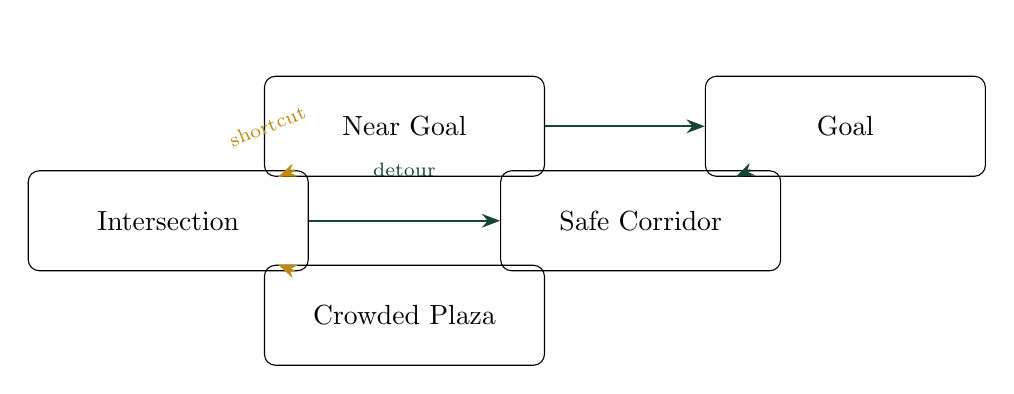
\begin{tikzpicture}[>=Stealth,every node/.style={draw,rounded corners,align=center,minimum width=1.4in,minimum height=0.5in}]
      \node (i) at (0,0) {Intersection};
      \node (n) at (3,1.2) {Near Goal};
      \node (c) at (3,-1.2) {Crowded Plaza};
      \node (s) at (6,0) {Safe Corridor};
      \node (g) at (8.6,1.2) {Goal};
      \draw[->,thick,CalPolyGold] (i)--node[draw=none,above,sloped]{\scriptsize shortcut} (n);
      \draw[->,thick,CalPolyGold] (i)--(c);
      \draw[->,thick,CalPolyGreen] (i)--node[draw=none,above]{\scriptsize detour} (s);
      \draw[->,thick,CalPolyGreen] (n)--(g);
      \draw[->,thick,CalPolyGreen] (s)--(g);
    \end{tikzpicture}
  \end{center}

  \begin{keyidea}
    An MDP graph represents possible state transitions; probabilities and rewards determine how attractive each branch is.
  \end{keyidea}
\end{frame}

\section{Long-Term Value}

% -----------------------------------------------------------------------------
% Slide 16
% -----------------------------------------------------------------------------
\begin{frame}[shrink=10]{Immediate Reward Can Choose the Wrong Action}
  Shortcut:
  \[
    R=+6
  \]
  Detour:
  \[
    R=+2
  \]

  A one-step agent prefers the shortcut immediately.

  But if the shortcut often enters a terrible future state, the correct long-run decision can reverse.

  \begin{keyidea}
    One-step expected utility becomes insufficient once the next state affects future opportunity.
  \end{keyidea}
\end{frame}

% -----------------------------------------------------------------------------
% Slide 17
% -----------------------------------------------------------------------------
\begin{frame}[shrink=10]{Action Value Adds the Future}
  \[
    Q(s,a)=\sum_{s'}T(s,a,s')\left[R(s,a,s')+\gamma V(s')\right]
  \]

  \begin{itemize}
    \item $T$: how likely is each next state?
    \item $R$: what do we receive now?
    \item $V(s')$: how good is the future state we create?
  \end{itemize}

  \begin{keyidea}
    An action is good when it gives good reward now and tends to place the robot in valuable future states.
  \end{keyidea}
\end{frame}

% -----------------------------------------------------------------------------
% Slide 18
% -----------------------------------------------------------------------------
\begin{frame}[shrink=10]{Bellman Optimality: The Core Recursion}
  \[
    V^*(s)=\max_a\sum_{s'}T(s,a,s')
    \left[R(s,a,s')+\gamma V^*(s')\right]
  \]

  Read it procedurally:
  \begin{enumerate}
    \item consider one candidate action;
    \item consider every next state it can produce;
    \item add immediate reward to discounted future value;
    \item average by transition probability;
    \item choose the action with the largest result.
  \end{enumerate}

  \begin{keyidea}
    The value of a state is the value of making the best first move and then behaving optimally afterward.
  \end{keyidea}
\end{frame}

% -----------------------------------------------------------------------------
% Slide 19
% -----------------------------------------------------------------------------
\begin{frame}[shrink=10]{Worked Comparison: Shortcut vs. Detour}
  Assume $\gamma=0.9$.

  Shortcut:
  \[
    Q=6+0.9[0.70(20)+0.30(-25)]=11.85
  \]

  Detour:
  \[
    Q=2+0.9[0.95(17)+0.05(-25)]=15.41
  \]

  \[
    \boxed{15.41>11.85}
  \]

  \begin{keyidea}
    The detour loses on immediate reward but wins after future consequences are included.
  \end{keyidea}
\end{frame}

% -----------------------------------------------------------------------------
% Slide 20
% -----------------------------------------------------------------------------
\begin{frame}[shrink=10]{What Is a Value Function?}
  \[
    V^\pi(s)=\mathbb{E}_\pi\left[G_t\mid S_t=s\right]
  \]

  $V^\pi(s)$ asks:
  \begin{quote}
    If I start in state $s$ and follow policy $\pi$ from now on, how much discounted reward should I expect?
  \end{quote}

  $V^*(s)$ asks the same question assuming optimal behavior from now on.

  \begin{keyidea}
    Values compress many possible future trajectories into one reusable number.
  \end{keyidea}
\end{frame}

% -----------------------------------------------------------------------------
% Slide 21
% -----------------------------------------------------------------------------
\begin{frame}[shrink=10]{Value Iteration: Repeated Bellman Backups}
  \[
    V_{k+1}(s)=\max_a\sum_{s'}T(s,a,s')
    \left[R(s,a,s')+\gamma V_k(s')\right]
  \]

  \begin{enumerate}
    \item initialize values, often $V_0(s)=0$;
    \item perform a Bellman backup for each state;
    \item repeat until values stabilize sufficiently.
  \end{enumerate}

  \begin{keyidea}
    Value iteration converts a long-horizon planning problem into repeated local updates.
  \end{keyidea}
\end{frame}

% -----------------------------------------------------------------------------
% Slide 22
% -----------------------------------------------------------------------------
\begin{frame}[shrink=10]{Intuition: Reward Propagates Backward}
  \begin{center}
    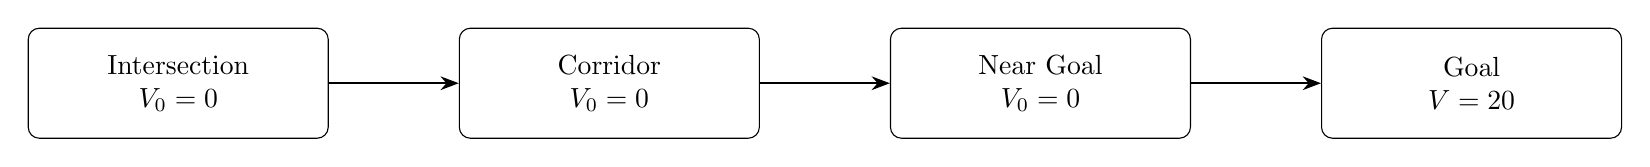
\begin{tikzpicture}[node distance=0.65in,every node/.style={draw,rounded corners,align=center,minimum width=1.5in,minimum height=0.55in}]
      \node (i) {Intersection\\$V_0=0$};
      \node[right=of i] (c) {Corridor\\$V_0=0$};
      \node[right=of c] (n) {Near Goal\\$V_0=0$};
      \node[right=of n] (g) {Goal\\$V=20$};
      \draw[-{Stealth},thick] (i)--(c);
      \draw[-{Stealth},thick] (c)--(n);
      \draw[-{Stealth},thick] (n)--(g);
    \end{tikzpicture}
  \end{center}

  Sweep 1 gives value to states near the goal. Later sweeps propagate that value farther backward.

  \begin{keyidea}
    Dynamic programming reuses downstream value estimates instead of enumerating every complete route.
  \end{keyidea}
\end{frame}

% -----------------------------------------------------------------------------
% Slide 23
% -----------------------------------------------------------------------------
\begin{frame}[shrink=10]{Extract the Policy from the Values}
  \[
    \pi^*(s)=\arg\max_a\sum_{s'}T(s,a,s')
    \left[R(s,a,s')+\gamma V^*(s')\right]
  \]

  Example policy:
  \begin{itemize}
    \item Intersection $\rightarrow$ Detour
    \item SafeCorridor $\rightarrow$ Forward
    \item CrowdedPlaza $\rightarrow$ Wait / Exit
    \item NearGoal $\rightarrow$ Deliver
  \end{itemize}

  \begin{keyidea}
    The value function scores states; the policy chooses the action that best exploits those values.
  \end{keyidea}
\end{frame}

% -----------------------------------------------------------------------------
% Slide 24
% -----------------------------------------------------------------------------
\begin{frame}[shrink=10]{Policy Iteration: Another Route to the Same Goal}
  \begin{columns}[T,onlytextwidth]
    \begin{column}{0.47\textwidth}
      \begin{block}{Policy evaluation}
        Hold a policy fixed and estimate how valuable every state is if the robot keeps following it.
      \end{block}
    \end{column}
    \begin{column}{0.47\textwidth}
      \begin{block}{Policy improvement}
        At each state, check whether a different action would produce greater expected long-term value.
      \end{block}
    \end{column}
  \end{columns}

  Repeat until the policy no longer changes.

  \begin{keyidea}
    Value iteration updates values directly; policy iteration alternates evaluating a policy and improving it.
  \end{keyidea}
\end{frame}

% -----------------------------------------------------------------------------
% Slide 25
% -----------------------------------------------------------------------------
\begin{frame}[shrink=10]{What an MDP Quietly Assumes}
  Standard MDP planning assumes:
  \begin{itemize}
    \item the current modeled state is known;
    \item a transition model is available;
    \item the state/action space is manageable enough to represent values or policies.
  \end{itemize}

  \begin{keyidea}
    MDPs solve sequential uncertainty in outcomes---but standard MDPs still assume the current state is observable.
  \end{keyidea}
\end{frame}

\section{Partial Observability}

% -----------------------------------------------------------------------------
% Slide 26
% -----------------------------------------------------------------------------
\begin{frame}[shrink=10]{And Here Is the Problem: The Robot Does Not Know the True State}
  \begin{itemize}
    \item the camera can miss pedestrians;
    \item LiDAR can be partially occluded;
    \item localization can drift;
    \item two hallways may look nearly identical;
    \item a door may be hidden around a corner.
  \end{itemize}

  \lectureimage[1.8in]{slide26.png}

  \begin{keyidea}
    The state that matters for planning can be hidden even when the robot has excellent sensors.
  \end{keyidea}
\end{frame}

% -----------------------------------------------------------------------------
% Slide 27
% -----------------------------------------------------------------------------
\begin{frame}[shrink=10]{Full Observability Was Doing More Work Than It Looked Like}
  An MDP policy is
  \[
    \pi(s).
  \]

  But the robot may only know
  \[
    P(CorridorA)=0.55,
    \qquad
    P(CorridorB)=0.45.
  \]

  Which state should we plug into the MDP policy?

  \begin{keyidea}
    If the current state is uncertain, a policy over physical states cannot be applied directly.
  \end{keyidea}
\end{frame}

% -----------------------------------------------------------------------------
% Slide 28
% -----------------------------------------------------------------------------
\begin{frame}[shrink=10]{But Lecture 21 Already Gave Us the Missing Object}
  \[
    b_t(s)=P(S_t=s\mid o_{1:t},a_{1:t-1})
  \]

  The \textbf{belief state} is a probability distribution over possible physical states.

  Example:
  \[
    b_t=[0.55,\;0.35,\;0.10]
  \]
  for Corridor A, Corridor B, and Plaza.

  \begin{keyidea}
    State estimation and sequential decision making meet at the belief state.
  \end{keyidea}
\end{frame}

% -----------------------------------------------------------------------------
% Slide 29
% -----------------------------------------------------------------------------
\begin{frame}[shrink=10]{Partially Observable Markov Decision Process}
  \[
    \boxed{POMDP=(S,A,T,R,\Omega,O,\gamma)}
  \]

  Relative to an MDP we add:
  \begin{itemize}
    \item $\Omega$: the possible observations;
    \item $O(o\mid s',a)$: the observation model.
  \end{itemize}

  \begin{keyidea}
    A POMDP is an MDP where the agent acts without directly observing the underlying state.
  \end{keyidea}
\end{frame}

% -----------------------------------------------------------------------------
% Slide 30
% -----------------------------------------------------------------------------
\begin{frame}[shrink=10]{The POMDP as a Dynamic Bayes Network}
  \begin{center}
    \begin{tikzpicture}[>=Stealth,node distance=0.9in,every node/.style={draw,rounded corners,align=center,minimum width=1.1in,minimum height=0.55in}]
      \node (s) {$S_t$};
      \node[right=of s] (a) {$A_t$};
      \node[right=of a] (sp) {$S_{t+1}$};
      \node[above right=0.5in and 0.9in of sp] (o) {$O_{t+1}$};
      \node[below right=0.5in and 0.9in of sp] (r) {$R_{t+1}$};
      \draw[->,thick] (s)--(sp);
      \draw[->,thick] (a)--(sp);
      \draw[->,thick] (sp)--(o);
      \draw[->,thick] (sp)--(r);
    \end{tikzpicture}
  \end{center}

  \begin{keyidea}
    The hidden state evolves, actions influence that evolution, and observations provide noisy evidence about the new state.
  \end{keyidea}
\end{frame}

% -----------------------------------------------------------------------------
% Slide 31
% -----------------------------------------------------------------------------
\begin{frame}[shrink=10]{The Belief State Becomes the Planning State}
  Physical state:
  \begin{quote}
    where the robot actually is, whether the route is truly blocked, whether a door is truly open.
  \end{quote}

  Belief state:
  \[
    b=[0.55,\;0.35,\;0.10].
  \]

  The controller now uses
  \[
    \pi(b)
  \]
  instead of $\pi(s)$.

  \begin{keyidea}
    The robot plans from a probability distribution rather than pretending one hidden state is certainly true.
  \end{keyidea}
\end{frame}

% -----------------------------------------------------------------------------
% Slide 32
% -----------------------------------------------------------------------------
\begin{frame}[shrink=10]{Belief Update: Predict, Then Correct}
  Prediction after action $a_t$:
  \[
    b^-_{t+1}(s')=\sum_s T(s,a_t,s')b_t(s).
  \]

  Correction after observation $o_{t+1}$:
  \[
    b_{t+1}(s')\propto O(o_{t+1}\mid s',a_t)b^-_{t+1}(s').
  \]

  \begin{keyidea}
    The POMDP belief update is the same predict--correct structure from filtering, now embedded inside decision making.
  \end{keyidea}
\end{frame}

% -----------------------------------------------------------------------------
% Slide 33
% -----------------------------------------------------------------------------
\begin{frame}[shrink=10]{The Elegant Trick: A POMDP Becomes an MDP over Beliefs}
  \begin{center}
    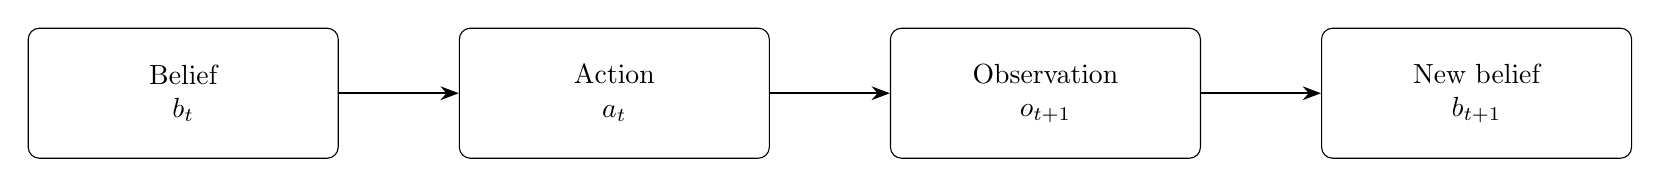
\begin{tikzpicture}[node distance=0.6in,every node/.style={draw,rounded corners,align=center,minimum width=1.55in,minimum height=0.65in}]
      \node (b) {Belief\\$b_t$};
      \node[right=of b] (a) {Action\\$a_t$};
      \node[right=of a] (o) {Observation\\$o_{t+1}$};
      \node[right=of o] (bp) {New belief\\$b_{t+1}$};
      \draw[-{Stealth},thick] (b)--(a);
      \draw[-{Stealth},thick] (a)--(o);
      \draw[-{Stealth},thick] (o)--(bp);
    \end{tikzpicture}
  \end{center}

  The full action/observation history can be compressed into the current belief.

  \begin{keyidea}
    The belief is a sufficient statistic for POMDP control---but that elegance creates a new computational problem.
  \end{keyidea}
\end{frame}

\section{Why POMDPs Blow Up}

% -----------------------------------------------------------------------------
% Slide 34
% -----------------------------------------------------------------------------
\begin{frame}[shrink=10]{Problem \#1: The Belief Space Is Continuous}
  Suppose there are only two possible hidden states: $A$ and $B$.

  A belief is
  \[
    b=[P(A),\;1-P(A)].
  \]

  Every value
  \[
    0\le P(A)\le1
  \]
  defines a different belief state.

  \begin{keyidea}
    Two physical states already create infinitely many possible beliefs.
  \end{keyidea}
\end{frame}

% -----------------------------------------------------------------------------
% Slide 35
% -----------------------------------------------------------------------------
\begin{frame}[shrink=10]{With Three Hidden States, Beliefs Fill a Triangle}
  For three hidden states,
  \[
    b=[p_1,p_2,p_3],
    \qquad
    p_1+p_2+p_3=1.
  \]

  \begin{center}
    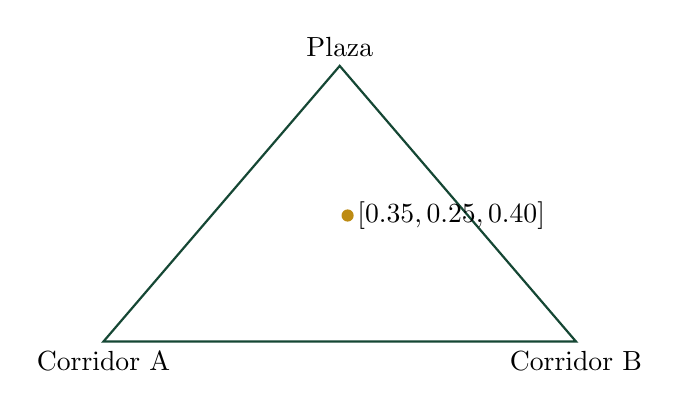
\begin{tikzpicture}
      \coordinate (a) at (0,0);
      \coordinate (b) at (6,0);
      \coordinate (c) at (3,3.5);
      \draw[thick,CalPolyGreen] (a)--(b)--(c)--cycle;
      \fill[CalPolyGold] (3.1,1.6) circle (2.2pt);
      \node[below] at (a) {Corridor A};
      \node[below] at (b) {Corridor B};
      \node[above] at (c) {Plaza};
      \node[right] at (3.1,1.6) {$[0.35,0.25,0.40]$};
    \end{tikzpicture}
  \end{center}

  \begin{keyidea}
    For $n$ hidden states, beliefs live in a continuous $(n-1)$-dimensional probability simplex.
  \end{keyidea}
\end{frame}

% -----------------------------------------------------------------------------
% Slide 36
% -----------------------------------------------------------------------------
\begin{frame}[shrink=10]{A POMDP Policy Maps Beliefs to Actions}
  Different belief regions can prefer different actions:
  \begin{itemize}
    \item highly confident in Corridor A $\rightarrow$ turn left;
    \item location ambiguous but uncertainty reducible $\rightarrow$ scan;
    \item likely near the plaza with high congestion $\rightarrow$ detour.
  \end{itemize}

  \begin{keyidea}
    The best action can change because the belief changes---even when the most likely physical state stays the same.
  \end{keyidea}
\end{frame}

% -----------------------------------------------------------------------------
% Slide 37
% -----------------------------------------------------------------------------
\begin{frame}[shrink=10]{Problem \#2: Future Observations Create Branching Contingencies}
  POMDP planning must reason about plans like:
  \begin{quote}
    Choose action $a_1$. If observation $o_1$ arrives, do $a_2$. If observation $o_2$ arrives instead, do $a_3$.
  \end{quote}

  So the future branches on:
  \begin{itemize}
    \item actions;
    \item stochastic physical transitions;
    \item stochastic observations;
    \item resulting belief updates.
  \end{itemize}

  \begin{keyidea}
    POMDP planning is contingency planning over both uncertain world evolution and uncertain future information.
  \end{keyidea}
\end{frame}

% -----------------------------------------------------------------------------
% Slide 38
% -----------------------------------------------------------------------------
\begin{frame}[shrink=10]{How Fast Does That Branching Grow?}
  A rough action--observation branching count is
  \[
    (|A||\Omega|)^H.
  \]

  With four actions, three coarse observation categories, and horizon $H=6$:
  \[
    (4\cdot3)^6=12^6\approx2.99\times10^6.
  \]

  And every branch carries a continuously valued belief distribution.

  \begin{keyidea}
    Horizon, action branching, observation branching, and continuous beliefs compound each other.
  \end{keyidea}
\end{frame}

\section{Back to Monte Carlo}

% -----------------------------------------------------------------------------
% Slide 39
% -----------------------------------------------------------------------------
\begin{frame}[shrink=10]{So We End Up Back at a Familiar Question}
  \begin{center}
    \Large\textbf{Do we really need to enumerate every possible future?}
  \end{center}

  \begin{columns}[T,onlytextwidth]
    \begin{column}{0.47\textwidth}
      \begin{block}{Exact approach}
        Represent and evaluate every relevant branch of the future.
      \end{block}
    \end{column}
    \begin{column}{0.47\textwidth}
      \begin{block}{Monte Carlo approach}
        Sample plausible futures, observe their returns, and estimate which actions look best.
      \end{block}
    \end{column}
  \end{columns}

  \begin{keyidea}
    The same tradeoff returns: give up exact enumeration to gain tractable approximate decision making.
  \end{keyidea}
\end{frame}

% -----------------------------------------------------------------------------
% Slide 40
% -----------------------------------------------------------------------------
\begin{frame}[shrink=10]{Monte Carlo Rollouts for Decision Making}
  A hand-wavy online planner can:
  \begin{enumerate}
    \item sample a physical state from the current belief;
    \item try a candidate action;
    \item sample the next state and observation;
    \item continue simulating a plausible future;
    \item accumulate discounted reward;
    \item repeat many times and average the return.
  \end{enumerate}

  \begin{keyidea}
    Monte Carlo planning estimates long-term action value from sampled futures instead of summing over all futures exactly.
  \end{keyidea}
\end{frame}

% -----------------------------------------------------------------------------
% Slide 41
% -----------------------------------------------------------------------------
\begin{frame}[shrink=10]{The Pieces We Already Learned Can Be Reused}
  \begin{columns}[T,onlytextwidth]
    \begin{column}{0.30\textwidth}
      \begin{block}{Particle belief}
        Represent the current belief with particles instead of an exact table.
      \end{block}
    \end{column}
    \begin{column}{0.30\textwidth}
      \begin{block}{Monte Carlo futures}
        Sample transitions and observations to generate possible trajectories.
      \end{block}
    \end{column}
    \begin{column}{0.30\textwidth}
      \begin{block}{Tree search}
        Spend more simulation on promising choices rather than exploring everything uniformly.
      \end{block}
    \end{column}
  \end{columns}

  \begin{keyidea}
    Approximate POMDP planning can combine sampled beliefs with Monte Carlo lookahead instead of constructing the entire belief-space solution.
  \end{keyidea}
\end{frame}

% -----------------------------------------------------------------------------
% Slide 42
% -----------------------------------------------------------------------------
\begin{frame}[shrink=10]{The Unit Has Come Full Circle}
  \begin{center}
    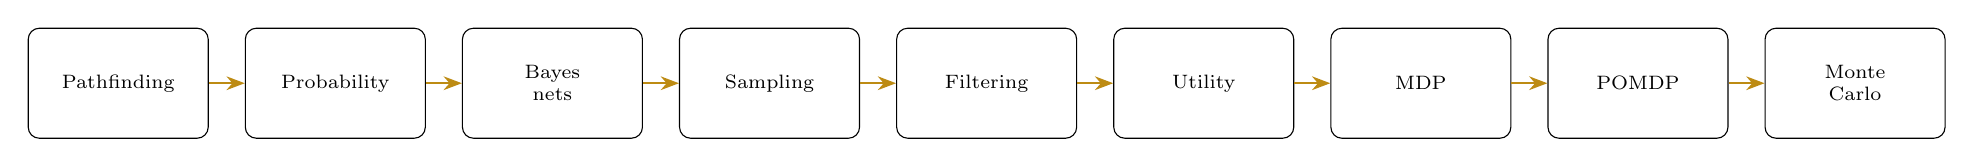
\begin{tikzpicture}[node distance=0.18in,every node/.style={draw,rounded corners,align=center,minimum width=0.9in,minimum height=0.55in,font=\scriptsize}]
      \node (p) {Pathfinding};
      \node[right=of p] (pr) {Probability};
      \node[right=of pr] (bn) {Bayes\\nets};
      \node[right=of bn] (samp) {Sampling};
      \node[right=of samp] (f) {Filtering};
      \node[right=of f] (u) {Utility};
      \node[right=of u] (m) {MDP};
      \node[right=of m] (po) {POMDP};
      \node[right=of po] (mc) {Monte\\Carlo};
      \foreach \x/\y in {p/pr,pr/bn,bn/samp,samp/f,f/u,u/m,m/po,po/mc}{\draw[-{Stealth},thick,CalPolyGold] (\x)--(\y);}
    \end{tikzpicture}
  \end{center}

  Each new model relaxes an assumption from the previous one---then pays for that flexibility with more computation.

  \begin{keyidea}
    AI repeatedly trades exactness, model simplicity, and computational cost to make rational decisions under real-world uncertainty.
  \end{keyidea}
\end{frame}

\end{document}
